% Options for packages loaded elsewhere
\PassOptionsToPackage{unicode}{hyperref}
\PassOptionsToPackage{hyphens}{url}
%
\documentclass[
]{article}
\title{Class16: RNASeq Mini Project}
\author{Yuhan Zhang (PID: A13829264)}
\date{11/19/2021}

\usepackage{amsmath,amssymb}
\usepackage{lmodern}
\usepackage{iftex}
\ifPDFTeX
  \usepackage[T1]{fontenc}
  \usepackage[utf8]{inputenc}
  \usepackage{textcomp} % provide euro and other symbols
\else % if luatex or xetex
  \usepackage{unicode-math}
  \defaultfontfeatures{Scale=MatchLowercase}
  \defaultfontfeatures[\rmfamily]{Ligatures=TeX,Scale=1}
\fi
% Use upquote if available, for straight quotes in verbatim environments
\IfFileExists{upquote.sty}{\usepackage{upquote}}{}
\IfFileExists{microtype.sty}{% use microtype if available
  \usepackage[]{microtype}
  \UseMicrotypeSet[protrusion]{basicmath} % disable protrusion for tt fonts
}{}
\makeatletter
\@ifundefined{KOMAClassName}{% if non-KOMA class
  \IfFileExists{parskip.sty}{%
    \usepackage{parskip}
  }{% else
    \setlength{\parindent}{0pt}
    \setlength{\parskip}{6pt plus 2pt minus 1pt}}
}{% if KOMA class
  \KOMAoptions{parskip=half}}
\makeatother
\usepackage{xcolor}
\IfFileExists{xurl.sty}{\usepackage{xurl}}{} % add URL line breaks if available
\IfFileExists{bookmark.sty}{\usepackage{bookmark}}{\usepackage{hyperref}}
\hypersetup{
  pdftitle={Class16: RNASeq Mini Project},
  pdfauthor={Yuhan Zhang (PID: A13829264)},
  hidelinks,
  pdfcreator={LaTeX via pandoc}}
\urlstyle{same} % disable monospaced font for URLs
\usepackage[margin=1in]{geometry}
\usepackage{color}
\usepackage{fancyvrb}
\newcommand{\VerbBar}{|}
\newcommand{\VERB}{\Verb[commandchars=\\\{\}]}
\DefineVerbatimEnvironment{Highlighting}{Verbatim}{commandchars=\\\{\}}
% Add ',fontsize=\small' for more characters per line
\usepackage{framed}
\definecolor{shadecolor}{RGB}{248,248,248}
\newenvironment{Shaded}{\begin{snugshade}}{\end{snugshade}}
\newcommand{\AlertTok}[1]{\textcolor[rgb]{0.94,0.16,0.16}{#1}}
\newcommand{\AnnotationTok}[1]{\textcolor[rgb]{0.56,0.35,0.01}{\textbf{\textit{#1}}}}
\newcommand{\AttributeTok}[1]{\textcolor[rgb]{0.77,0.63,0.00}{#1}}
\newcommand{\BaseNTok}[1]{\textcolor[rgb]{0.00,0.00,0.81}{#1}}
\newcommand{\BuiltInTok}[1]{#1}
\newcommand{\CharTok}[1]{\textcolor[rgb]{0.31,0.60,0.02}{#1}}
\newcommand{\CommentTok}[1]{\textcolor[rgb]{0.56,0.35,0.01}{\textit{#1}}}
\newcommand{\CommentVarTok}[1]{\textcolor[rgb]{0.56,0.35,0.01}{\textbf{\textit{#1}}}}
\newcommand{\ConstantTok}[1]{\textcolor[rgb]{0.00,0.00,0.00}{#1}}
\newcommand{\ControlFlowTok}[1]{\textcolor[rgb]{0.13,0.29,0.53}{\textbf{#1}}}
\newcommand{\DataTypeTok}[1]{\textcolor[rgb]{0.13,0.29,0.53}{#1}}
\newcommand{\DecValTok}[1]{\textcolor[rgb]{0.00,0.00,0.81}{#1}}
\newcommand{\DocumentationTok}[1]{\textcolor[rgb]{0.56,0.35,0.01}{\textbf{\textit{#1}}}}
\newcommand{\ErrorTok}[1]{\textcolor[rgb]{0.64,0.00,0.00}{\textbf{#1}}}
\newcommand{\ExtensionTok}[1]{#1}
\newcommand{\FloatTok}[1]{\textcolor[rgb]{0.00,0.00,0.81}{#1}}
\newcommand{\FunctionTok}[1]{\textcolor[rgb]{0.00,0.00,0.00}{#1}}
\newcommand{\ImportTok}[1]{#1}
\newcommand{\InformationTok}[1]{\textcolor[rgb]{0.56,0.35,0.01}{\textbf{\textit{#1}}}}
\newcommand{\KeywordTok}[1]{\textcolor[rgb]{0.13,0.29,0.53}{\textbf{#1}}}
\newcommand{\NormalTok}[1]{#1}
\newcommand{\OperatorTok}[1]{\textcolor[rgb]{0.81,0.36,0.00}{\textbf{#1}}}
\newcommand{\OtherTok}[1]{\textcolor[rgb]{0.56,0.35,0.01}{#1}}
\newcommand{\PreprocessorTok}[1]{\textcolor[rgb]{0.56,0.35,0.01}{\textit{#1}}}
\newcommand{\RegionMarkerTok}[1]{#1}
\newcommand{\SpecialCharTok}[1]{\textcolor[rgb]{0.00,0.00,0.00}{#1}}
\newcommand{\SpecialStringTok}[1]{\textcolor[rgb]{0.31,0.60,0.02}{#1}}
\newcommand{\StringTok}[1]{\textcolor[rgb]{0.31,0.60,0.02}{#1}}
\newcommand{\VariableTok}[1]{\textcolor[rgb]{0.00,0.00,0.00}{#1}}
\newcommand{\VerbatimStringTok}[1]{\textcolor[rgb]{0.31,0.60,0.02}{#1}}
\newcommand{\WarningTok}[1]{\textcolor[rgb]{0.56,0.35,0.01}{\textbf{\textit{#1}}}}
\usepackage{graphicx}
\makeatletter
\def\maxwidth{\ifdim\Gin@nat@width>\linewidth\linewidth\else\Gin@nat@width\fi}
\def\maxheight{\ifdim\Gin@nat@height>\textheight\textheight\else\Gin@nat@height\fi}
\makeatother
% Scale images if necessary, so that they will not overflow the page
% margins by default, and it is still possible to overwrite the defaults
% using explicit options in \includegraphics[width, height, ...]{}
\setkeys{Gin}{width=\maxwidth,height=\maxheight,keepaspectratio}
% Set default figure placement to htbp
\makeatletter
\def\fps@figure{htbp}
\makeatother
\setlength{\emergencystretch}{3em} % prevent overfull lines
\providecommand{\tightlist}{%
  \setlength{\itemsep}{0pt}\setlength{\parskip}{0pt}}
\setcounter{secnumdepth}{-\maxdimen} % remove section numbering
\ifLuaTeX
  \usepackage{selnolig}  % disable illegal ligatures
\fi

\begin{document}
\maketitle

\begin{Shaded}
\begin{Highlighting}[]
\FunctionTok{library}\NormalTok{(DESeq2)}
\end{Highlighting}
\end{Shaded}

\hypertarget{data-import}{%
\section{1. Data Import}\label{data-import}}

Load data:

\begin{Shaded}
\begin{Highlighting}[]
\NormalTok{metaFile }\OtherTok{\textless{}{-}} \StringTok{"GSE37704\_metadata.csv"}
\NormalTok{countFile }\OtherTok{\textless{}{-}} \StringTok{"GSE37704\_featurecounts.csv"}
\end{Highlighting}
\end{Shaded}

\begin{Shaded}
\begin{Highlighting}[]
\NormalTok{colData }\OtherTok{\textless{}{-}} \FunctionTok{read.csv}\NormalTok{(metaFile, }\AttributeTok{row.names =} \DecValTok{1}\NormalTok{)}
\FunctionTok{head}\NormalTok{(colData)}
\end{Highlighting}
\end{Shaded}

\begin{verbatim}
##               condition
## SRR493366 control_sirna
## SRR493367 control_sirna
## SRR493368 control_sirna
## SRR493369      hoxa1_kd
## SRR493370      hoxa1_kd
## SRR493371      hoxa1_kd
\end{verbatim}

\begin{Shaded}
\begin{Highlighting}[]
\NormalTok{countData }\OtherTok{\textless{}{-}} \FunctionTok{read.csv}\NormalTok{(countFile, }\AttributeTok{row.names =} \DecValTok{1}\NormalTok{)}
\FunctionTok{head}\NormalTok{(countData)}
\end{Highlighting}
\end{Shaded}

\begin{verbatim}
##                 length SRR493366 SRR493367 SRR493368 SRR493369 SRR493370
## ENSG00000186092    918         0         0         0         0         0
## ENSG00000279928    718         0         0         0         0         0
## ENSG00000279457   1982        23        28        29        29        28
## ENSG00000278566    939         0         0         0         0         0
## ENSG00000273547    939         0         0         0         0         0
## ENSG00000187634   3214       124       123       205       207       212
##                 SRR493371
## ENSG00000186092         0
## ENSG00000279928         0
## ENSG00000279457        46
## ENSG00000278566         0
## ENSG00000273547         0
## ENSG00000187634       258
\end{verbatim}

We need to remove the first column (i.e.~\texttt{countData\$length}) to
match with metadata:

\begin{Shaded}
\begin{Highlighting}[]
\NormalTok{countData }\OtherTok{\textless{}{-}} \FunctionTok{as.matrix}\NormalTok{(countData[, }\SpecialCharTok{{-}}\DecValTok{1}\NormalTok{])}
\FunctionTok{head}\NormalTok{(countData)}
\end{Highlighting}
\end{Shaded}

\begin{verbatim}
##                 SRR493366 SRR493367 SRR493368 SRR493369 SRR493370 SRR493371
## ENSG00000186092         0         0         0         0         0         0
## ENSG00000279928         0         0         0         0         0         0
## ENSG00000279457        23        28        29        29        28        46
## ENSG00000278566         0         0         0         0         0         0
## ENSG00000273547         0         0         0         0         0         0
## ENSG00000187634       124       123       205       207       212       258
\end{verbatim}

We also need to remove entries that has no reading (0 across all
columns)

\begin{Shaded}
\begin{Highlighting}[]
\NormalTok{row.rm }\OtherTok{=} \FunctionTok{rowSums}\NormalTok{(countData) }\SpecialCharTok{!=} \DecValTok{0}
\NormalTok{countData }\OtherTok{\textless{}{-}}\NormalTok{ countData[row.rm,]}
\FunctionTok{head}\NormalTok{(countData)}
\end{Highlighting}
\end{Shaded}

\begin{verbatim}
##                 SRR493366 SRR493367 SRR493368 SRR493369 SRR493370 SRR493371
## ENSG00000279457        23        28        29        29        28        46
## ENSG00000187634       124       123       205       207       212       258
## ENSG00000188976      1637      1831      2383      1226      1326      1504
## ENSG00000187961       120       153       180       236       255       357
## ENSG00000187583        24        48        65        44        48        64
## ENSG00000187642         4         9        16        14        16        16
\end{verbatim}

\begin{Shaded}
\begin{Highlighting}[]
\FunctionTok{nrow}\NormalTok{(countData)}
\end{Highlighting}
\end{Shaded}

\begin{verbatim}
## [1] 15975
\end{verbatim}

\hypertarget{pca-for-quality-control}{%
\section{2. PCA for Quality Control}\label{pca-for-quality-control}}

\begin{Shaded}
\begin{Highlighting}[]
\NormalTok{pca }\OtherTok{\textless{}{-}} \FunctionTok{prcomp}\NormalTok{(}\FunctionTok{t}\NormalTok{(countData))}
\FunctionTok{summary}\NormalTok{(pca)}
\end{Highlighting}
\end{Shaded}

\begin{verbatim}
## Importance of components:
##                              PC1       PC2       PC3       PC4      PC5
## Standard deviation     1.852e+05 1.001e+05 1.998e+04 6.886e+03 5.15e+03
## Proportion of Variance 7.659e-01 2.235e-01 8.920e-03 1.060e-03 5.90e-04
## Cumulative Proportion  7.659e-01 9.894e-01 9.983e-01 9.994e-01 1.00e+00
##                              PC6
## Standard deviation     9.558e-10
## Proportion of Variance 0.000e+00
## Cumulative Proportion  1.000e+00
\end{verbatim}

Plot first and second:

\begin{Shaded}
\begin{Highlighting}[]
\FunctionTok{plot}\NormalTok{(pca}\SpecialCharTok{$}\NormalTok{x)}
\end{Highlighting}
\end{Shaded}

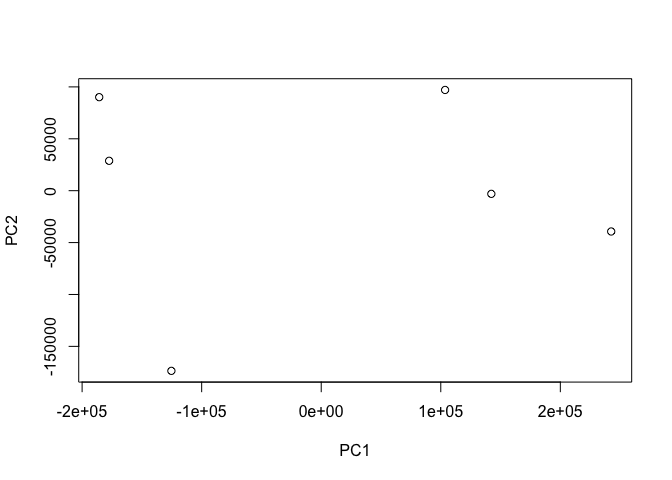
\includegraphics{class16_files/figure-latex/unnamed-chunk-9-1.pdf}

\begin{Shaded}
\begin{Highlighting}[]
\FunctionTok{plot}\NormalTok{(pca}\SpecialCharTok{$}\NormalTok{x[, }\DecValTok{1}\SpecialCharTok{:}\DecValTok{2}\NormalTok{], }\AttributeTok{pch =} \DecValTok{16}\NormalTok{, }\AttributeTok{col =} \FunctionTok{as.factor}\NormalTok{(colData}\SpecialCharTok{$}\NormalTok{condition))}
\FunctionTok{text}\NormalTok{(pca}\SpecialCharTok{$}\NormalTok{x[, }\DecValTok{1}\SpecialCharTok{:}\DecValTok{2}\NormalTok{], }\AttributeTok{labels =}\NormalTok{ colData}\SpecialCharTok{$}\NormalTok{condition)}
\end{Highlighting}
\end{Shaded}

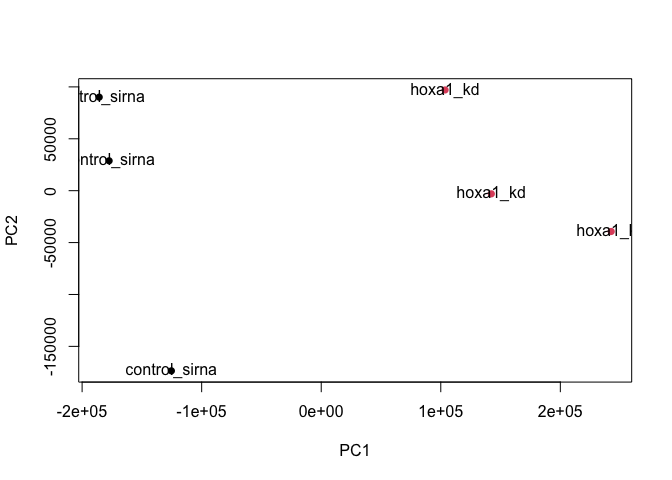
\includegraphics{class16_files/figure-latex/unnamed-chunk-10-1.pdf}

ggplot version:

\begin{Shaded}
\begin{Highlighting}[]
\FunctionTok{library}\NormalTok{(ggplot2)}

\NormalTok{x }\OtherTok{\textless{}{-}} \FunctionTok{as.data.frame}\NormalTok{(pca}\SpecialCharTok{$}\NormalTok{x)}
\NormalTok{x}\SpecialCharTok{$}\NormalTok{condition }\OtherTok{\textless{}{-}}\NormalTok{ colData}\SpecialCharTok{$}\NormalTok{condition}

\FunctionTok{ggplot}\NormalTok{(x, }\FunctionTok{aes}\NormalTok{(PC1, PC2, }\AttributeTok{col=}\NormalTok{condition)) }\SpecialCharTok{+} 
  \FunctionTok{geom\_point}\NormalTok{()}
\end{Highlighting}
\end{Shaded}

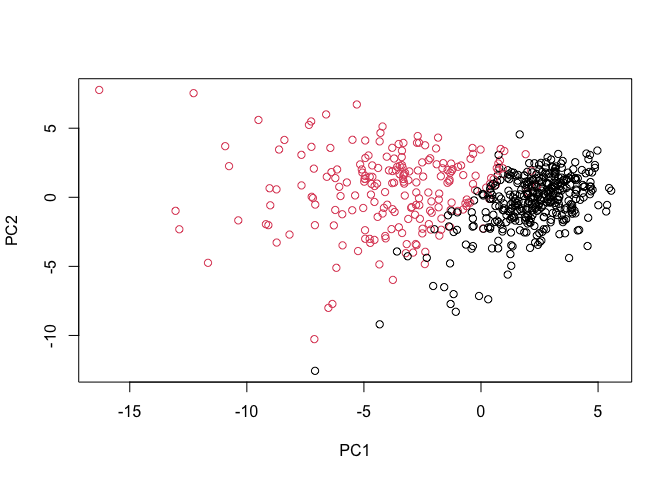
\includegraphics{class16_files/figure-latex/unnamed-chunk-11-1.pdf}

\hypertarget{running-deseq2}{%
\section{3. Running DESeq2}\label{running-deseq2}}

\begin{Shaded}
\begin{Highlighting}[]
\NormalTok{dds }\OtherTok{\textless{}{-}} \FunctionTok{DESeqDataSetFromMatrix}\NormalTok{(}\AttributeTok{countData =}\NormalTok{ countData, }
                             \AttributeTok{colData =}\NormalTok{ colData, }
                             \AttributeTok{design =} \SpecialCharTok{\textasciitilde{}}\NormalTok{condition)}
\end{Highlighting}
\end{Shaded}

\begin{verbatim}
## Warning in DESeqDataSet(se, design = design, ignoreRank): some variables in
## design formula are characters, converting to factors
\end{verbatim}

\begin{Shaded}
\begin{Highlighting}[]
\NormalTok{dds }\OtherTok{\textless{}{-}} \FunctionTok{DESeq}\NormalTok{(dds)}
\end{Highlighting}
\end{Shaded}

\begin{verbatim}
## estimating size factors
\end{verbatim}

\begin{verbatim}
## estimating dispersions
\end{verbatim}

\begin{verbatim}
## gene-wise dispersion estimates
\end{verbatim}

\begin{verbatim}
## mean-dispersion relationship
\end{verbatim}

\begin{verbatim}
## final dispersion estimates
\end{verbatim}

\begin{verbatim}
## fitting model and testing
\end{verbatim}

\begin{Shaded}
\begin{Highlighting}[]
\NormalTok{dds}
\end{Highlighting}
\end{Shaded}

\begin{verbatim}
## class: DESeqDataSet 
## dim: 15975 6 
## metadata(1): version
## assays(4): counts mu H cooks
## rownames(15975): ENSG00000279457 ENSG00000187634 ... ENSG00000276345
##   ENSG00000271254
## rowData names(22): baseMean baseVar ... deviance maxCooks
## colnames(6): SRR493366 SRR493367 ... SRR493370 SRR493371
## colData names(2): condition sizeFactor
\end{verbatim}

Get result from our DESeq data:

\begin{Shaded}
\begin{Highlighting}[]
\NormalTok{res }\OtherTok{\textless{}{-}}  \FunctionTok{results}\NormalTok{(dds)}
\end{Highlighting}
\end{Shaded}

\begin{Shaded}
\begin{Highlighting}[]
\FunctionTok{summary}\NormalTok{(res)}
\end{Highlighting}
\end{Shaded}

\begin{verbatim}
## 
## out of 15975 with nonzero total read count
## adjusted p-value < 0.1
## LFC > 0 (up)       : 4349, 27%
## LFC < 0 (down)     : 4396, 28%
## outliers [1]       : 0, 0%
## low counts [2]     : 1237, 7.7%
## (mean count < 0)
## [1] see 'cooksCutoff' argument of ?results
## [2] see 'independentFiltering' argument of ?results
\end{verbatim}

\hypertarget{volcano-plot}{%
\section{4. Volcano Plot}\label{volcano-plot}}

Let's do the classic log2-FoldChange vs p-value volcano plot

\begin{Shaded}
\begin{Highlighting}[]
\FunctionTok{plot}\NormalTok{(res}\SpecialCharTok{$}\NormalTok{log2FoldChange, }\SpecialCharTok{{-}}\FunctionTok{log}\NormalTok{(res}\SpecialCharTok{$}\NormalTok{padj))}
\end{Highlighting}
\end{Shaded}

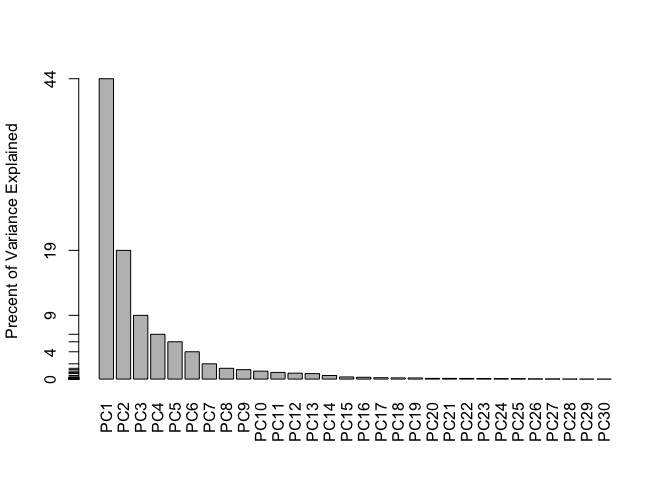
\includegraphics{class16_files/figure-latex/unnamed-chunk-16-1.pdf}

Add color

\begin{Shaded}
\begin{Highlighting}[]
\NormalTok{mycol }\OtherTok{\textless{}{-}} \FunctionTok{rep}\NormalTok{(}\StringTok{"gray"}\NormalTok{, }\FunctionTok{nrow}\NormalTok{(res))}
\NormalTok{mycol[}\FunctionTok{abs}\NormalTok{(res}\SpecialCharTok{$}\NormalTok{log2FoldChange) }\SpecialCharTok{\textgreater{}} \DecValTok{2}\NormalTok{] }\OtherTok{\textless{}{-}} \StringTok{"blue"}
\NormalTok{mycol[res}\SpecialCharTok{$}\NormalTok{padj }\SpecialCharTok{\textgreater{}} \FloatTok{0.05} \SpecialCharTok{\&} \FunctionTok{abs}\NormalTok{(res}\SpecialCharTok{$}\NormalTok{log2FoldChange) }\SpecialCharTok{\textgreater{}} \DecValTok{2}\NormalTok{] }\OtherTok{\textless{}{-}} \StringTok{"red"}

\FunctionTok{plot}\NormalTok{(res}\SpecialCharTok{$}\NormalTok{log2FoldChange, }\SpecialCharTok{{-}}\FunctionTok{log}\NormalTok{(res}\SpecialCharTok{$}\NormalTok{padj), }\AttributeTok{col =}\NormalTok{ mycol, }\AttributeTok{xlab =} \StringTok{"log2(FoldChange)"}\NormalTok{, }
     \AttributeTok{ylab =} \StringTok{"{-}log(p{-}value"}\NormalTok{)}
\end{Highlighting}
\end{Shaded}

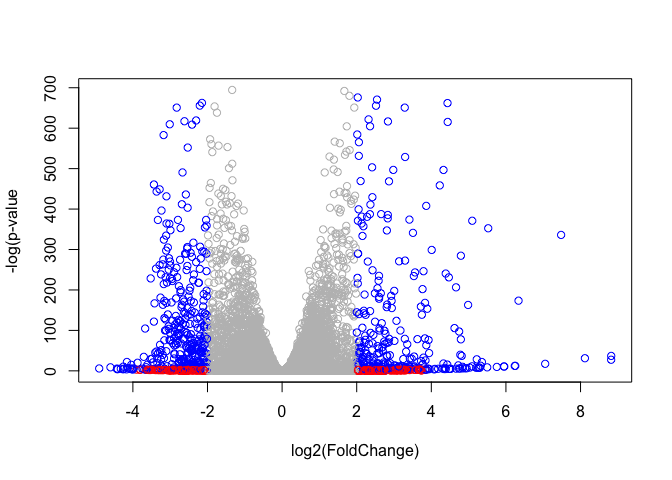
\includegraphics{class16_files/figure-latex/unnamed-chunk-17-1.pdf}

\hypertarget{annotation}{%
\section{5. Annotation}\label{annotation}}

\begin{Shaded}
\begin{Highlighting}[]
\FunctionTok{library}\NormalTok{(}\StringTok{"AnnotationDbi"}\NormalTok{)}
\end{Highlighting}
\end{Shaded}

\begin{verbatim}
## Warning: package 'AnnotationDbi' was built under R version 4.1.2
\end{verbatim}

\begin{Shaded}
\begin{Highlighting}[]
\FunctionTok{library}\NormalTok{(}\StringTok{"org.Hs.eg.db"}\NormalTok{)}
\end{Highlighting}
\end{Shaded}

\begin{Shaded}
\begin{Highlighting}[]
\FunctionTok{columns}\NormalTok{(org.Hs.eg.db)}
\end{Highlighting}
\end{Shaded}

\begin{verbatim}
##  [1] "ACCNUM"       "ALIAS"        "ENSEMBL"      "ENSEMBLPROT"  "ENSEMBLTRANS"
##  [6] "ENTREZID"     "ENZYME"       "EVIDENCE"     "EVIDENCEALL"  "GENENAME"    
## [11] "GENETYPE"     "GO"           "GOALL"        "IPI"          "MAP"         
## [16] "OMIM"         "ONTOLOGY"     "ONTOLOGYALL"  "PATH"         "PFAM"        
## [21] "PMID"         "PROSITE"      "REFSEQ"       "SYMBOL"       "UCSCKG"      
## [26] "UNIPROT"
\end{verbatim}

\begin{Shaded}
\begin{Highlighting}[]
\NormalTok{res}\SpecialCharTok{$}\NormalTok{symbol }\OtherTok{=} \FunctionTok{mapIds}\NormalTok{(org.Hs.eg.db,}
                    \AttributeTok{keys=}\FunctionTok{row.names}\NormalTok{(res), }
                    \AttributeTok{keytype=}\StringTok{"ENSEMBL"}\NormalTok{,}
                    \AttributeTok{column=}\StringTok{"SYMBOL"}\NormalTok{,}
                    \AttributeTok{multiVals=}\StringTok{"first"}\NormalTok{)}
\end{Highlighting}
\end{Shaded}

\begin{verbatim}
## 'select()' returned 1:many mapping between keys and columns
\end{verbatim}

\begin{Shaded}
\begin{Highlighting}[]
\NormalTok{res}\SpecialCharTok{$}\NormalTok{entrez }\OtherTok{=} \FunctionTok{mapIds}\NormalTok{(org.Hs.eg.db,}
                    \AttributeTok{keys=}\FunctionTok{row.names}\NormalTok{(res),}
                    \AttributeTok{keytype=}\StringTok{"ENSEMBL"}\NormalTok{,}
                    \AttributeTok{column=}\StringTok{"ENTREZID"}\NormalTok{,}
                    \AttributeTok{multiVals=}\StringTok{"first"}\NormalTok{)}
\end{Highlighting}
\end{Shaded}

\begin{verbatim}
## 'select()' returned 1:many mapping between keys and columns
\end{verbatim}

\begin{Shaded}
\begin{Highlighting}[]
\NormalTok{res}\SpecialCharTok{$}\NormalTok{name }\OtherTok{=}   \FunctionTok{mapIds}\NormalTok{(org.Hs.eg.db,}
                    \AttributeTok{keys=}\FunctionTok{row.names}\NormalTok{(res),}
                    \AttributeTok{keytype=}\StringTok{"ENSEMBL"}\NormalTok{,}
                    \AttributeTok{column=}\StringTok{"GENENAME"}\NormalTok{,}
                    \AttributeTok{multiVals=}\StringTok{"first"}\NormalTok{)}
\end{Highlighting}
\end{Shaded}

\begin{verbatim}
## 'select()' returned 1:many mapping between keys and columns
\end{verbatim}

\begin{Shaded}
\begin{Highlighting}[]
\FunctionTok{head}\NormalTok{(res, }\DecValTok{10}\NormalTok{)}
\end{Highlighting}
\end{Shaded}

\begin{verbatim}
## log2 fold change (MLE): condition hoxa1 kd vs control sirna 
## Wald test p-value: condition hoxa1 kd vs control sirna 
## DataFrame with 10 rows and 9 columns
##                    baseMean log2FoldChange     lfcSE       stat      pvalue
##                   <numeric>      <numeric> <numeric>  <numeric>   <numeric>
## ENSG00000279457   29.913579      0.1792571 0.3248216   0.551863 5.81042e-01
## ENSG00000187634  183.229650      0.4264571 0.1402658   3.040350 2.36304e-03
## ENSG00000188976 1651.188076     -0.6927205 0.0548465 -12.630158 1.43990e-36
## ENSG00000187961  209.637938      0.7297556 0.1318599   5.534326 3.12428e-08
## ENSG00000187583   47.255123      0.0405765 0.2718928   0.149237 8.81366e-01
## ENSG00000187642   11.979750      0.5428105 0.5215598   1.040744 2.97994e-01
## ENSG00000188290  108.922128      2.0570638 0.1969053  10.446970 1.51282e-25
## ENSG00000187608  350.716868      0.2573837 0.1027266   2.505522 1.22271e-02
## ENSG00000188157 9128.439422      0.3899088 0.0467163   8.346304 7.04321e-17
## ENSG00000237330    0.158192      0.7859552 4.0804729   0.192614 8.47261e-01
##                        padj      symbol      entrez                   name
##                   <numeric> <character> <character>            <character>
## ENSG00000279457 6.86555e-01      WASH9P   102723897 WAS protein family h..
## ENSG00000187634 5.15718e-03      SAMD11      148398 sterile alpha motif ..
## ENSG00000188976 1.76549e-35       NOC2L       26155 NOC2 like nucleolar ..
## ENSG00000187961 1.13413e-07      KLHL17      339451 kelch like family me..
## ENSG00000187583 9.19031e-01     PLEKHN1       84069 pleckstrin homology ..
## ENSG00000187642 4.03379e-01       PERM1       84808 PPARGC1 and ESRR ind..
## ENSG00000188290 1.30538e-24        HES4       57801 hes family bHLH tran..
## ENSG00000187608 2.37452e-02       ISG15        9636 ISG15 ubiquitin like..
## ENSG00000188157 4.21963e-16        AGRN      375790                  agrin
## ENSG00000237330          NA      RNF223      401934 ring finger protein ..
\end{verbatim}

\hypertarget{pathway-analysis}{%
\section{6. Pathway Analysis}\label{pathway-analysis}}

Use KEGG pathways:

\begin{Shaded}
\begin{Highlighting}[]
\FunctionTok{library}\NormalTok{(pathview)}
\FunctionTok{library}\NormalTok{(gage)}
\FunctionTok{library}\NormalTok{(gageData)}
\end{Highlighting}
\end{Shaded}

\begin{Shaded}
\begin{Highlighting}[]
\FunctionTok{data}\NormalTok{(kegg.sets.hs)}
\FunctionTok{data}\NormalTok{(sigmet.idx.hs)}

\CommentTok{\# Focus on signaling and metabolic pathways only}
\NormalTok{kegg.sets.hs }\OtherTok{=}\NormalTok{ kegg.sets.hs[sigmet.idx.hs]}

\CommentTok{\# Examine the first 3 pathways}
\FunctionTok{head}\NormalTok{(kegg.sets.hs, }\DecValTok{3}\NormalTok{)}
\end{Highlighting}
\end{Shaded}

\begin{verbatim}
## $`hsa00232 Caffeine metabolism`
## [1] "10"   "1544" "1548" "1549" "1553" "7498" "9"   
## 
## $`hsa00983 Drug metabolism - other enzymes`
##  [1] "10"     "1066"   "10720"  "10941"  "151531" "1548"   "1549"   "1551"  
##  [9] "1553"   "1576"   "1577"   "1806"   "1807"   "1890"   "221223" "2990"  
## [17] "3251"   "3614"   "3615"   "3704"   "51733"  "54490"  "54575"  "54576" 
## [25] "54577"  "54578"  "54579"  "54600"  "54657"  "54658"  "54659"  "54963" 
## [33] "574537" "64816"  "7083"   "7084"   "7172"   "7363"   "7364"   "7365"  
## [41] "7366"   "7367"   "7371"   "7372"   "7378"   "7498"   "79799"  "83549" 
## [49] "8824"   "8833"   "9"      "978"   
## 
## $`hsa00230 Purine metabolism`
##   [1] "100"    "10201"  "10606"  "10621"  "10622"  "10623"  "107"    "10714" 
##   [9] "108"    "10846"  "109"    "111"    "11128"  "11164"  "112"    "113"   
##  [17] "114"    "115"    "122481" "122622" "124583" "132"    "158"    "159"   
##  [25] "1633"   "171568" "1716"   "196883" "203"    "204"    "205"    "221823"
##  [33] "2272"   "22978"  "23649"  "246721" "25885"  "2618"   "26289"  "270"   
##  [41] "271"    "27115"  "272"    "2766"   "2977"   "2982"   "2983"   "2984"  
##  [49] "2986"   "2987"   "29922"  "3000"   "30833"  "30834"  "318"    "3251"  
##  [57] "353"    "3614"   "3615"   "3704"   "377841" "471"    "4830"   "4831"  
##  [65] "4832"   "4833"   "4860"   "4881"   "4882"   "4907"   "50484"  "50940" 
##  [73] "51082"  "51251"  "51292"  "5136"   "5137"   "5138"   "5139"   "5140"  
##  [81] "5141"   "5142"   "5143"   "5144"   "5145"   "5146"   "5147"   "5148"  
##  [89] "5149"   "5150"   "5151"   "5152"   "5153"   "5158"   "5167"   "5169"  
##  [97] "51728"  "5198"   "5236"   "5313"   "5315"   "53343"  "54107"  "5422"  
## [105] "5424"   "5425"   "5426"   "5427"   "5430"   "5431"   "5432"   "5433"  
## [113] "5434"   "5435"   "5436"   "5437"   "5438"   "5439"   "5440"   "5441"  
## [121] "5471"   "548644" "55276"  "5557"   "5558"   "55703"  "55811"  "55821" 
## [129] "5631"   "5634"   "56655"  "56953"  "56985"  "57804"  "58497"  "6240"  
## [137] "6241"   "64425"  "646625" "654364" "661"    "7498"   "8382"   "84172" 
## [145] "84265"  "84284"  "84618"  "8622"   "8654"   "87178"  "8833"   "9060"  
## [153] "9061"   "93034"  "953"    "9533"   "954"    "955"    "956"    "957"   
## [161] "9583"   "9615"
\end{verbatim}

Make the input foldchange vector for KEGG and GO:

\begin{Shaded}
\begin{Highlighting}[]
\NormalTok{foldchanges }\OtherTok{=}\NormalTok{ res}\SpecialCharTok{$}\NormalTok{log2FoldChange}
\FunctionTok{names}\NormalTok{(foldchanges) }\OtherTok{=}\NormalTok{ res}\SpecialCharTok{$}\NormalTok{entrez}
\FunctionTok{head}\NormalTok{(foldchanges)}
\end{Highlighting}
\end{Shaded}

\begin{verbatim}
##   102723897      148398       26155      339451       84069       84808 
##  0.17925708  0.42645712 -0.69272046  0.72975561  0.04057653  0.54281049
\end{verbatim}

\begin{Shaded}
\begin{Highlighting}[]
\CommentTok{\# Get the results}
\NormalTok{keggres }\OtherTok{=} \FunctionTok{gage}\NormalTok{(foldchanges, }\AttributeTok{gsets=}\NormalTok{kegg.sets.hs)}
\end{Highlighting}
\end{Shaded}

Look at the object return from \texttt{gage()}

\begin{Shaded}
\begin{Highlighting}[]
\FunctionTok{attributes}\NormalTok{(keggres)}
\end{Highlighting}
\end{Shaded}

\begin{verbatim}
## $names
## [1] "greater" "less"    "stats"
\end{verbatim}

Downregulated pathway:

\begin{Shaded}
\begin{Highlighting}[]
\CommentTok{\# Look at the first few down (less) pathways}
\FunctionTok{head}\NormalTok{(keggres}\SpecialCharTok{$}\NormalTok{less)}
\end{Highlighting}
\end{Shaded}

\begin{verbatim}
##                                          p.geomean stat.mean        p.val
## hsa04110 Cell cycle                   8.995727e-06 -4.378644 8.995727e-06
## hsa03030 DNA replication              9.424076e-05 -3.951803 9.424076e-05
## hsa03013 RNA transport                1.246882e-03 -3.059466 1.246882e-03
## hsa03440 Homologous recombination     3.066756e-03 -2.852899 3.066756e-03
## hsa04114 Oocyte meiosis               3.784520e-03 -2.698128 3.784520e-03
## hsa00010 Glycolysis / Gluconeogenesis 8.961413e-03 -2.405398 8.961413e-03
##                                             q.val set.size         exp1
## hsa04110 Cell cycle                   0.001448312      121 8.995727e-06
## hsa03030 DNA replication              0.007586381       36 9.424076e-05
## hsa03013 RNA transport                0.066915974      144 1.246882e-03
## hsa03440 Homologous recombination     0.121861535       28 3.066756e-03
## hsa04114 Oocyte meiosis               0.121861535      102 3.784520e-03
## hsa00010 Glycolysis / Gluconeogenesis 0.212222694       53 8.961413e-03
\end{verbatim}

Let's look at the first downregulated pathway:

\begin{Shaded}
\begin{Highlighting}[]
\FunctionTok{pathview}\NormalTok{(}\AttributeTok{gene.data=}\NormalTok{foldchanges, }\AttributeTok{pathway.id=}\StringTok{"hsa04110"}\NormalTok{)}
\end{Highlighting}
\end{Shaded}

\begin{verbatim}
## 'select()' returned 1:1 mapping between keys and columns
\end{verbatim}

\begin{verbatim}
## Info: Working in directory /Users/deka/Dropbox/My Mac (ciaiqinmachudeMacBook-Pro.local)/Documents/BGGN213_R/bggn213/class16
\end{verbatim}

\begin{verbatim}
## Info: Writing image file hsa04110.pathview.png
\end{verbatim}

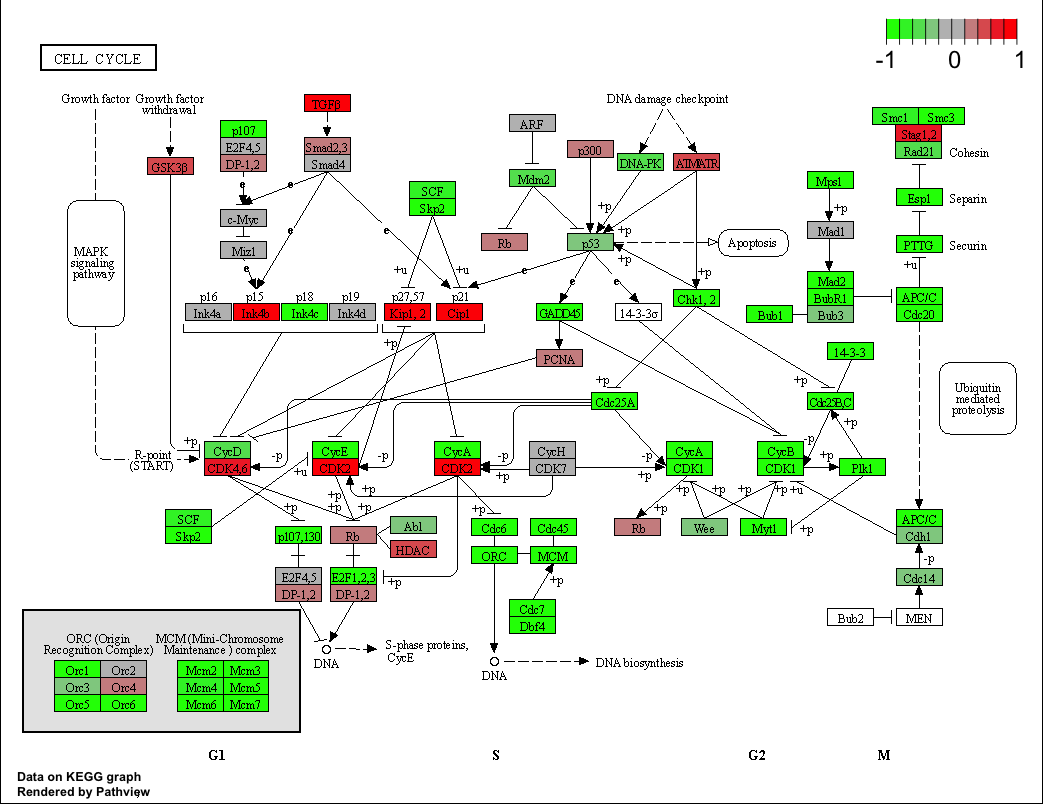
\includegraphics{hsa04110.pathview.png}

We can automatically pull up 5 upregulated pathway by doing so

\begin{Shaded}
\begin{Highlighting}[]
\NormalTok{keggrespathways }\OtherTok{\textless{}{-}} \FunctionTok{rownames}\NormalTok{(keggres}\SpecialCharTok{$}\NormalTok{greater)[}\DecValTok{1}\SpecialCharTok{:}\DecValTok{5}\NormalTok{]}

\NormalTok{keggresids }\OtherTok{=} \FunctionTok{substr}\NormalTok{(keggrespathways, }\AttributeTok{start=}\DecValTok{1}\NormalTok{, }\AttributeTok{stop=}\DecValTok{8}\NormalTok{)}
\NormalTok{keggresids}
\end{Highlighting}
\end{Shaded}

\begin{verbatim}
## [1] "hsa04640" "hsa04630" "hsa00140" "hsa04142" "hsa04330"
\end{verbatim}

\begin{Shaded}
\begin{Highlighting}[]
\FunctionTok{pathview}\NormalTok{(}\AttributeTok{gene.data=}\NormalTok{foldchanges, }\AttributeTok{pathway.id=}\NormalTok{keggresids, }\AttributeTok{species=}\StringTok{"hsa"}\NormalTok{)}
\end{Highlighting}
\end{Shaded}

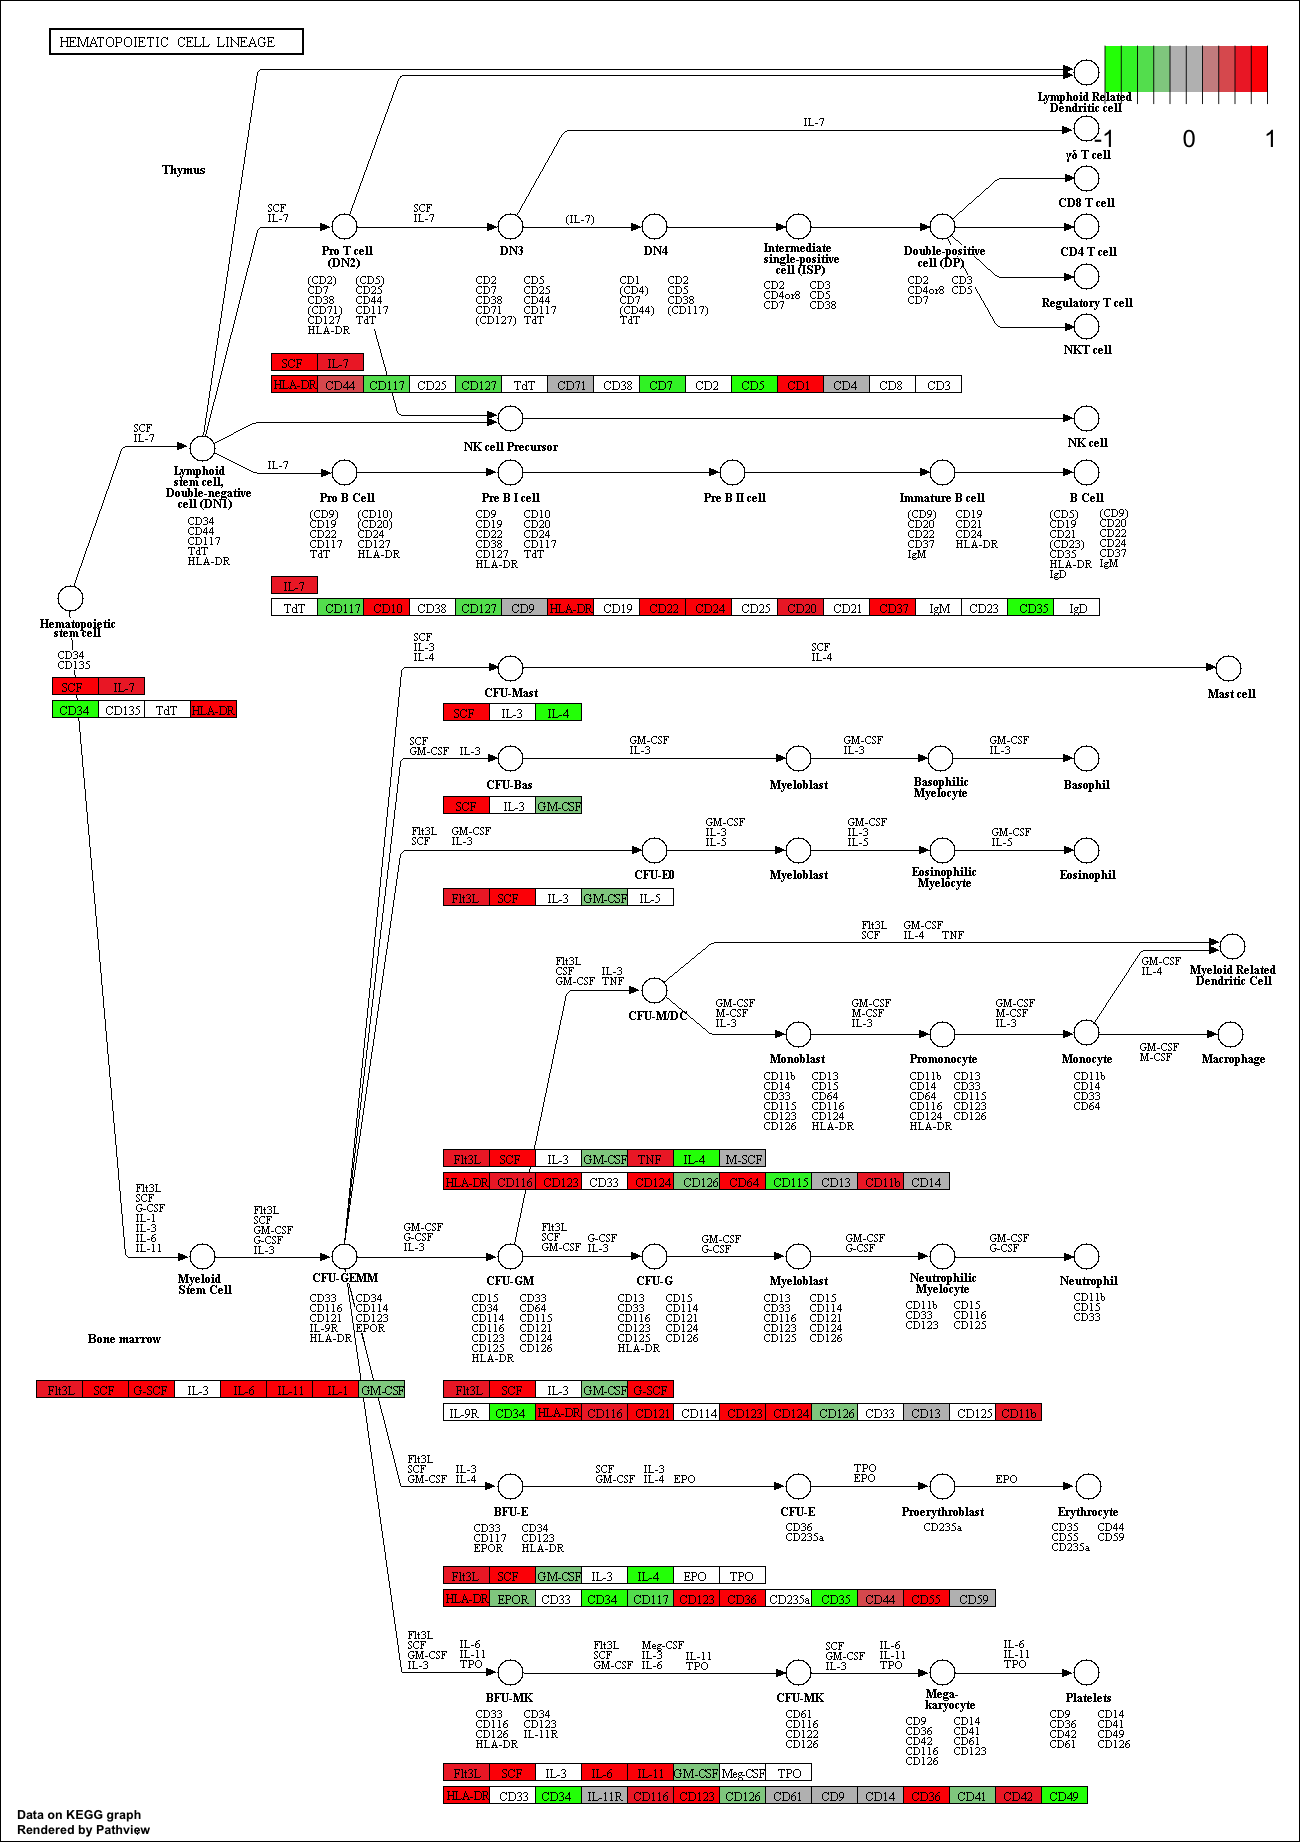
\includegraphics{hsa04640.pathview.png}
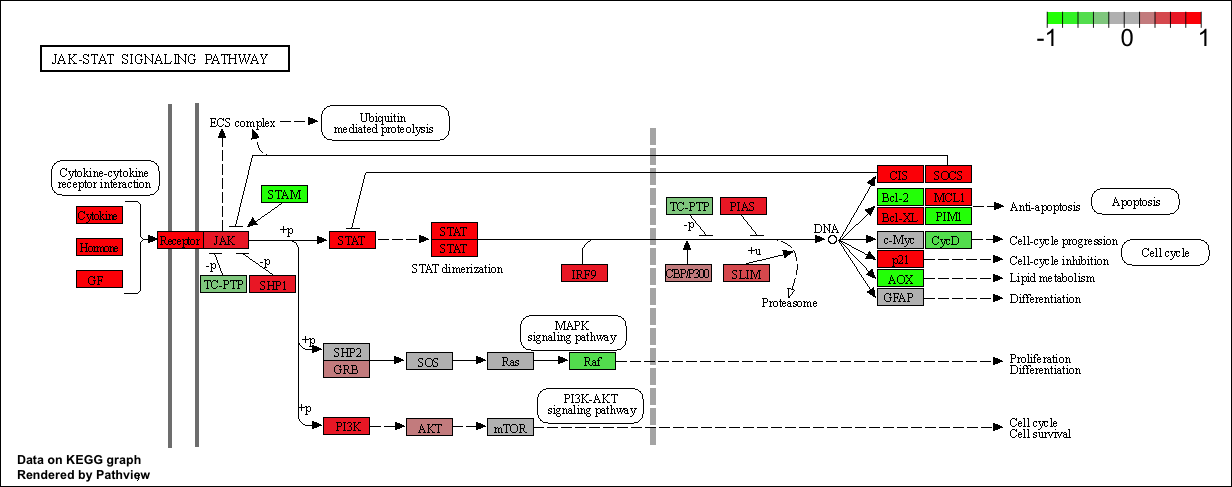
\includegraphics{hsa04630.pathview.png}
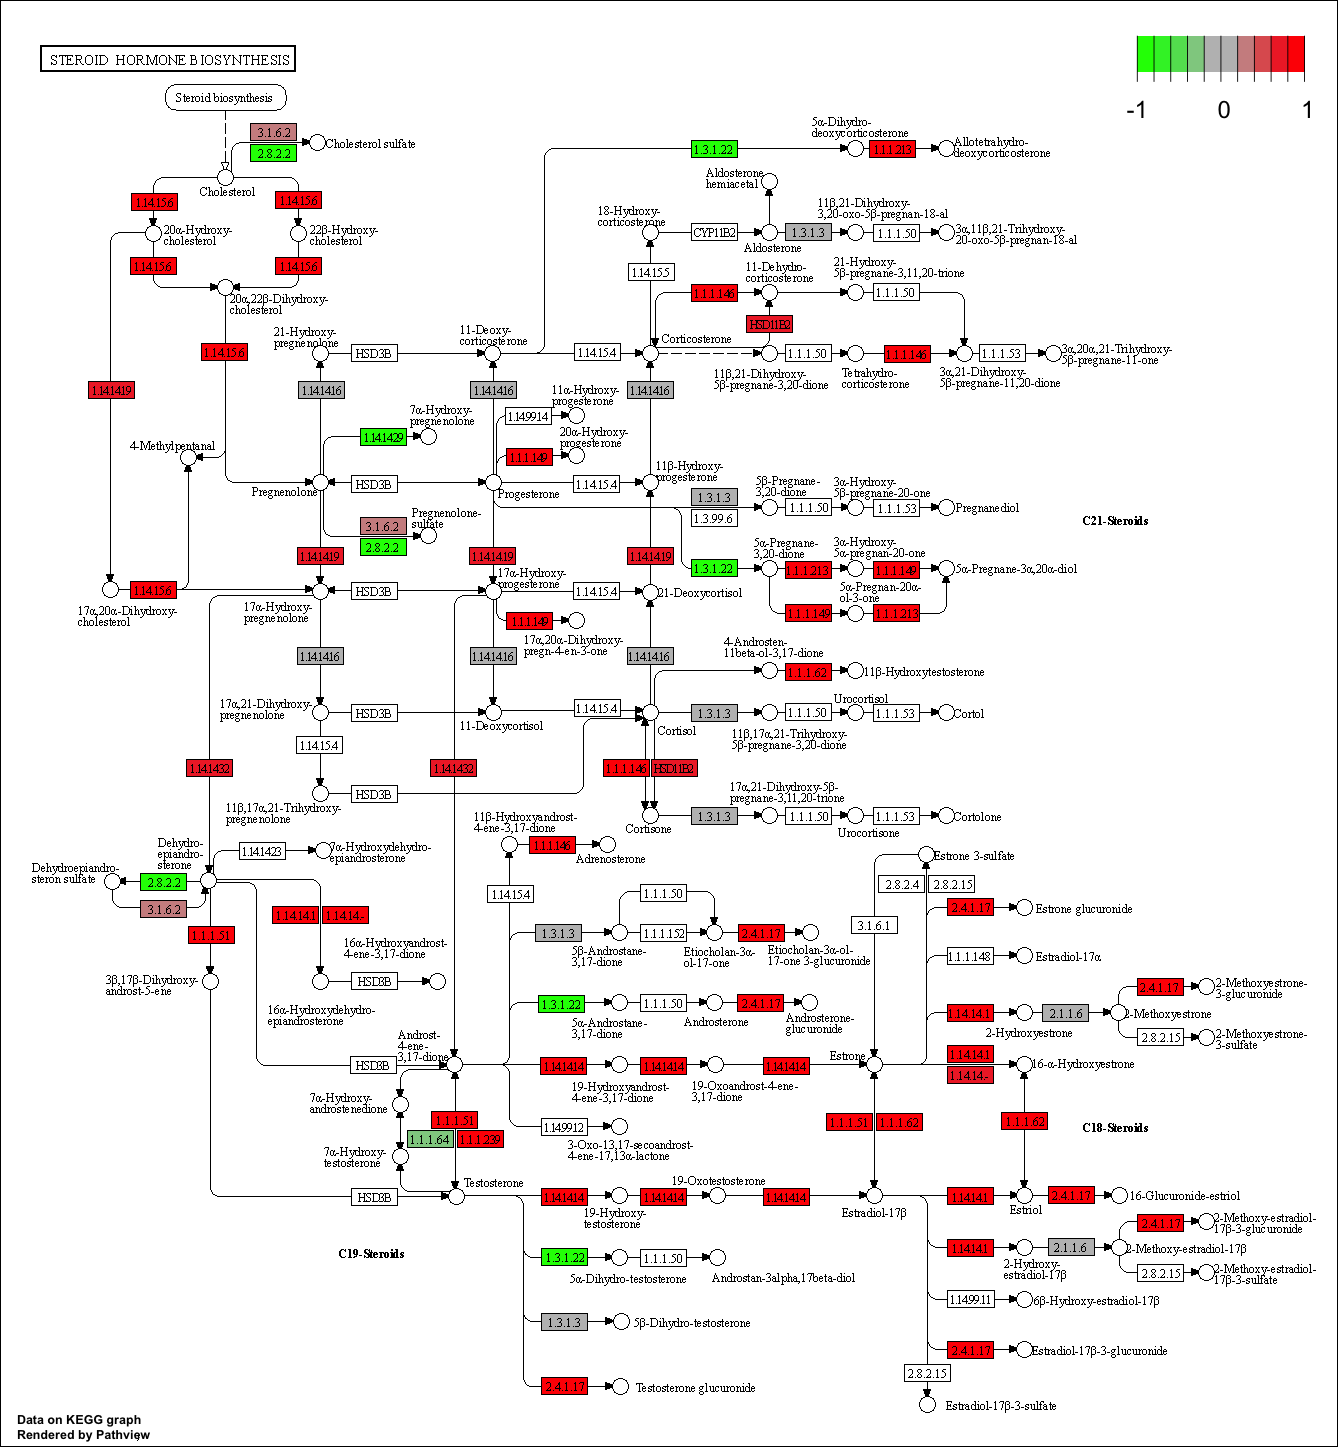
\includegraphics{hsa00140.pathview.png}
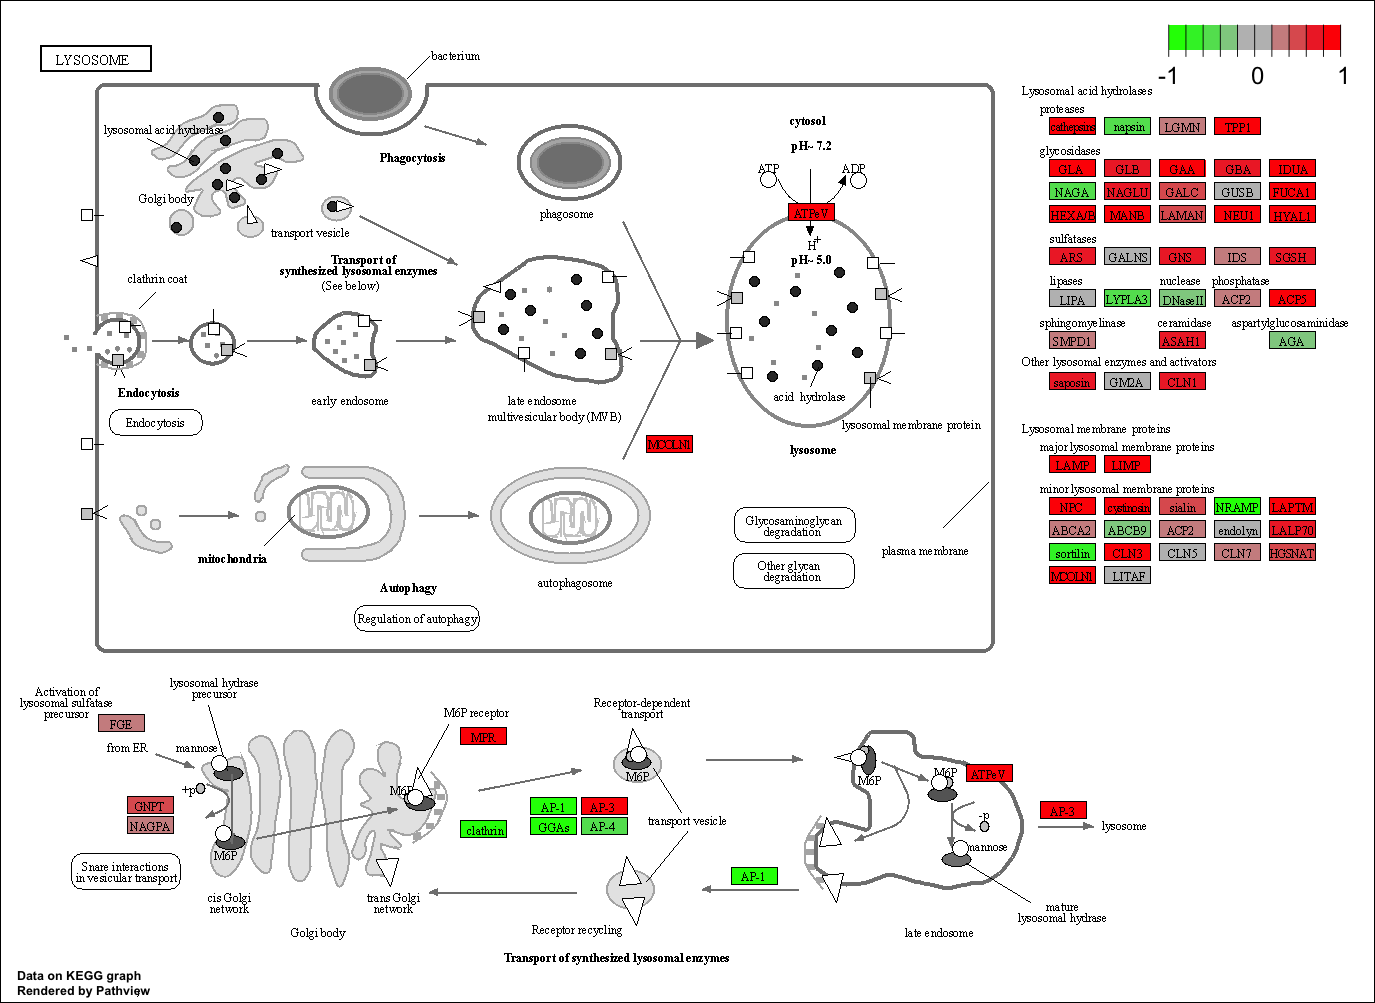
\includegraphics{hsa04142.pathview.png}
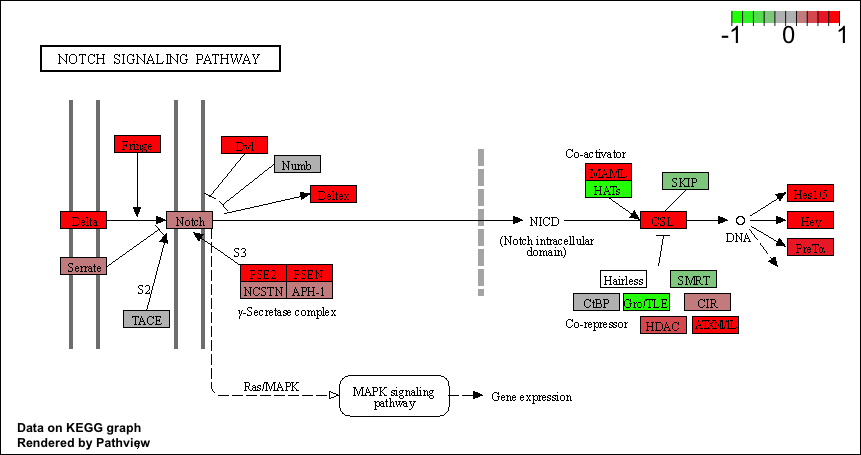
\includegraphics{hsa04330.pathview.png}

We can also do similar thing using gene ontology. Focus on biological
process:

\begin{Shaded}
\begin{Highlighting}[]
\FunctionTok{data}\NormalTok{(go.sets.hs)}
\FunctionTok{data}\NormalTok{(go.subs.hs)}

\CommentTok{\# Focus on Biological Process subset of GO}
\NormalTok{gobpsets }\OtherTok{=}\NormalTok{ go.sets.hs[go.subs.hs}\SpecialCharTok{$}\NormalTok{BP]}

\NormalTok{gobpres }\OtherTok{=} \FunctionTok{gage}\NormalTok{(foldchanges, }\AttributeTok{gsets=}\NormalTok{gobpsets, }\AttributeTok{same.dir=}\ConstantTok{TRUE}\NormalTok{)}

\FunctionTok{lapply}\NormalTok{(gobpres, head)}
\end{Highlighting}
\end{Shaded}

\begin{verbatim}
## $greater
##                                              p.geomean stat.mean        p.val
## GO:0007156 homophilic cell adhesion       8.519724e-05  3.824205 8.519724e-05
## GO:0002009 morphogenesis of an epithelium 1.396681e-04  3.653886 1.396681e-04
## GO:0048729 tissue morphogenesis           1.432451e-04  3.643242 1.432451e-04
## GO:0007610 behavior                       2.195494e-04  3.530241 2.195494e-04
## GO:0060562 epithelial tube morphogenesis  5.932837e-04  3.261376 5.932837e-04
## GO:0035295 tube development               5.953254e-04  3.253665 5.953254e-04
##                                               q.val set.size         exp1
## GO:0007156 homophilic cell adhesion       0.1951953      113 8.519724e-05
## GO:0002009 morphogenesis of an epithelium 0.1951953      339 1.396681e-04
## GO:0048729 tissue morphogenesis           0.1951953      424 1.432451e-04
## GO:0007610 behavior                       0.2243795      427 2.195494e-04
## GO:0060562 epithelial tube morphogenesis  0.3711390      257 5.932837e-04
## GO:0035295 tube development               0.3711390      391 5.953254e-04
## 
## $less
##                                             p.geomean stat.mean        p.val
## GO:0048285 organelle fission             1.536227e-15 -8.063910 1.536227e-15
## GO:0000280 nuclear division              4.286961e-15 -7.939217 4.286961e-15
## GO:0007067 mitosis                       4.286961e-15 -7.939217 4.286961e-15
## GO:0000087 M phase of mitotic cell cycle 1.169934e-14 -7.797496 1.169934e-14
## GO:0007059 chromosome segregation        2.028624e-11 -6.878340 2.028624e-11
## GO:0000236 mitotic prometaphase          1.729553e-10 -6.695966 1.729553e-10
##                                                 q.val set.size         exp1
## GO:0048285 organelle fission             5.841698e-12      376 1.536227e-15
## GO:0000280 nuclear division              5.841698e-12      352 4.286961e-15
## GO:0007067 mitosis                       5.841698e-12      352 4.286961e-15
## GO:0000087 M phase of mitotic cell cycle 1.195672e-11      362 1.169934e-14
## GO:0007059 chromosome segregation        1.658603e-08      142 2.028624e-11
## GO:0000236 mitotic prometaphase          1.178402e-07       84 1.729553e-10
## 
## $stats
##                                           stat.mean     exp1
## GO:0007156 homophilic cell adhesion        3.824205 3.824205
## GO:0002009 morphogenesis of an epithelium  3.653886 3.653886
## GO:0048729 tissue morphogenesis            3.643242 3.643242
## GO:0007610 behavior                        3.530241 3.530241
## GO:0060562 epithelial tube morphogenesis   3.261376 3.261376
## GO:0035295 tube development                3.253665 3.253665
\end{verbatim}

\end{document}
